% \begin{table*}[!ht]
% \setlength{\tabcolsep}{6pt}
% \centering
% % \vspace{-10pt}
% \caption{Domain adaptation results.}
%   % \vspace{-8pt}
%   \begin{adjustbox}{width=0.979\textwidth}
%   \input{tables/table1}
%   \end{adjustbox}
%   % \vskip -0.14in
%   % % \vspace{-6pt}
% \label{tab:heart}
% % \tabcolsep2pt
% \end{table*}

\section{Experiments}
% We conducted extensive evaluations of our multi-matching approach on two 2D segmentation benchmark tasks: optic disc and cup segmentation in retinal fundus images, and polyp segmentation datasets.

\subsection{Datasets}

\textbf{The retinal fundus segmentation datasets} comprise five public datasets from different medical centers, denoted as Site A (RIM-ONE~\cite{fumero2011rim}), B (REFUGE~\cite{orlando2020refuge}), C (ORIGA~\cite{zhang2010origa}), D (REFUGE-Test~\cite{orlando2020refuge}), and E (Drishti-GS~\cite{sivaswamy2014drishti}), with 159, 400, 650, 800, and 101 images respectively, all consistently annotated for optic disc (OD) and optic cup (OC) segmentation. We adopted the preprocessing method outlined in~\cite{liu2022single,chen2024each}, where each image's region of interest is cropped to $800\times800$ pixels and normalized using min-max normalization.

\noindent \textbf{The polyp segmentation datasets} consist of four public datasets collected from different medical centers, denoted as Site A (BKAI-IGH-NEOPolyp~\cite{ngoc2021neounet}), B (CVC-ClinicDB/CVC-612~\cite{bernal2015wm}), C (ETIS~\cite{silva2014toward}), and D (Kvasir~\cite{jha2020kvasir}), containing 1000, 612, 196, and 1000 images, respectively. We followed the preprocessing steps in~\cite{chen2024each}, resizing the images to $800 \times 800$ pixels and normalizing them using ImageNet-derived statistics.

\subsection{Experimental Setup}
\label{exp_setup}
\textbf{Implementation Details.} To ensure a fair comparison across all methods, we followed the protocol in~\cite{chen2024each} and split each dataset into an $8:2$ ratio for training and testing. We employed the ResNet-50~\cite{he2016deep} pre-trained on ImageNet as the feature extractor. The training was optimized using the SGD optimizer with a momentum of 0.9 and a learning rate of 0.001. For source model training, we set the mini-batch size to 8, allowing simultaneous matching of 8 graphs per batch. The universe embedding $\mathcal{U}$ was treated as an additional trainable tensor, integrated into the network weights without influencing subsequent experiments with other methods.
During the TTA phase, all methods were trained on the target data without access to their labels. The mini-batch size was set to 4, and the previously learned $\mathcal{U}$ from source model training was frozen. All experiments were implemented using PyTorch and conducted on 4 NVIDIA 3090 GPUs.

\noindent \textbf{Evaluation Metrics.} The Dice score (DSC, \%) was used to quantify the accuracy of the predicted masks, serving as the primary metric for evaluating segmentation performance. Additionally, the enhanced alignment metric $E_\phi^{max}$~\cite{fan2018enhanced} was adopted to measure both pixel-level and global-level similarity. To further assess the consistency between predictions and ground truths, we also employed the structural similarity metric $S_{\alpha}$~\cite{fan2017structure}.

\subsection{Experimental Results}
We selected U-Net~\cite{ronneberger2015u} as the benchmark model for the segmentation task, training it on the source domains and testing on the target domain without adaptation (\textit{No Adapt}). In addition, we compared eight state-of-the-art (SOTA) methods, including two entropy-based approaches (TENT~\cite{wangtent} and SAR~\cite{niu2023towards}), a shape template-based method (TASD~\cite{liu2022single}), a dynamically adjusted learning rate method (DLTTA~\cite{yang2022dltta}), batch normalization-based methods (DomainAdaptor~\cite{zhang2023domainadaptor}, VPTTA~\cite{chen2024each}), and noise estimation-based approaches (DeY-Net~\cite{wen2024denoising} and NC-TTT~\cite{osowiechi2024nc}).


\begin{table*}[h!]
% \vspace{-9pt}
% \setlength{\tabcolsep}{1pt}
\centering
  \caption{Multi sources domain generaliation in retinal fundus segmentation. The average performance (mean $\pm$ standard deviation) of three trials for our method and nine SOTA methods. ``Site A'' means training on Sites B-E and testing on Site A, and similarly for the others. The best results are highlighted in \textcolor{red}{red}.}
  \vspace{-5pt}
  \begin{adjustbox}{width=0.99\linewidth}
    \begin{tabular}{c|ccccccccccccccc|ccc}
\hlineB{3}
\multirow{2}{*}{Methods} & \multicolumn{3}{c}{Site A} & \multicolumn{3}{c}{Site B} & \multicolumn{3}{c}{Site C} & \multicolumn{3}{c}{Site D} & \multicolumn{3}{c|}{Site E} & \multicolumn{3}{c}{Average} \\ \cline{2-19} 
                         & \textit{DSC}       & $E_\phi^{max}$       & $S_{\alpha}$      & \textit{DSC}       & $E_\phi^{max}$       & $S_{\alpha}$     & \textit{DSC}       & $E_\phi^{max}$       & $S_{\alpha}$    & \textit{DSC}       & $E_\phi^{max}$       & $S_{\alpha}$  & \textit{DSC}       & $E_\phi^{max}$       & $S_{\alpha}$      & \textit{DSC} $\uparrow$      & $E_\phi^{max}$ $\uparrow$       & $S_{\alpha}$ $\uparrow$    \\ \hline \hline
\textit{No Adapt} (U-Net~\cite{ronneberger2015u}) & 65.60\small{$\pm$5.78} & 91.75\small{$\pm$0.13} & 79.11\small{$\pm$0.07} & 74.65\small{$\pm$4.88} & 88.78\small{$\pm$0.08} & 83.31\small{$\pm$0.02} & 63.15\small{$\pm$7.30} & 81.03\small{$\pm$0.19} & 79.77\small{$\pm$0.03} & 68.11\small{$\pm$5.49} & 89.46\small{$\pm$0.20} & 82.12\small{$\pm$0.07} & 75.34\small{$\pm$1.01} & 90.68\small{$\pm$0.16} & 87.53\small{$\pm$0.05} & 69.37 & 88.34 & 82.36 \\ \hline
TENT (ICLR'21)~\cite{wangtent} & 75.22\small{$\pm$3.99} & \textcolor{red}{94.10\small{$\pm$0.10}} & 83.97\small{$\pm$0.05} & 81.06\small{$\pm$0.93} & 93.45\small{$\pm$0.11} & \textcolor{red}{92.36\small{$\pm$0.03}} &  75.23\small{$\pm$2.33} & 88.10\small{$\pm$0.14} & 84.62\small{$\pm$0.03} & 78.12\small{$\pm$2.59} & 91.33\small{$\pm$0.31} & 86.41\small{$\pm$0.12}  & 83.17\small{$\pm$0.78} & 92.74\small{$\pm$0.10} & 93.64\small{$\pm$0.03} & 78.56 & 91.94 & 88.20     \\
TASD (AAAI'22)~\cite{liu2022single} & 79.70\small{$\pm$2.52} & 88.73\small{$\pm$0.45} & 83.67\small{$\pm$0.17} & 82.96\small{$\pm$2.14} & 94.01\small{$\pm$0.20} & 90.99\small{$\pm$0.11} & 86.12\small{$\pm$1.11} & 93.59\small{$\pm$0.13} & 87.08\small{$\pm$0.07} & 78.02\small{$\pm$6.30} & 87.20\small{$\pm$0.16} & 87.94\small{$\pm$0.04} & 83.71\small{$\pm$3.77} & 90.88\small{$\pm$0.25} & 90.37\small{$\pm$0.12} & 82.10 & 90.88 & 88.01 \\
% CoTTA (CVPR'22)~\cite{wang2022continual}       \\

DLTTA (TMI'22)~\cite{yang2022dltta} & 71.88\small{$\pm$5.59} & 86.29\small{$\pm$0.21} & 80.70\small{$\pm$0.13} & 80.12\small{$\pm$2.26} & 90.53\small{$\pm$0.17} & 88.63\small{$\pm$0.06} & 81.46\small{$\pm$3.35} & 93.08\small{$\pm$0.08} & 87.48\small{$\pm$0.02} & 75.90\small{$\pm$7.27} & 84.27\small{$\pm$0.12} & 84.79\small{$\pm$0.06} & 82.75\small{$\pm$6.55} & 90.10\small{$\pm$0.31} & 89.33\small{$\pm$0.14} & 78.42 & 88.85 & 86.18 \\

SAR (ICLR'23)~\cite{niu2023towards} & 75.29\small{$\pm$2.69} & 88.73\small{$\pm$0.34} & 80.15\small{$\pm$0.26} & 86.42\small{$\pm$1.57} & 96.88\small{$\pm$0.27} & 91.28\small{$\pm$0.09} & 80.69\small{$\pm$4.30} & 92.10\small{$\pm$0.15} & 86.31\small{$\pm$0.27} & 80.27\small{$\pm$5.47} & 89.98\small{$\pm$0.31} & 87.20\small{$\pm$0.15} & 89.61\small{$\pm$0.28} & 95.90\small{$\pm$0.08} & 92.06\small{$\pm$0.01} & 82.46 & 92.71 & 87.40\\

DomainAdaptor (CVPR'23)~\cite{zhang2023domainadaptor} & 77.14\small{$\pm$1.21} & 90.80\small{$\pm$0.19} & 81.31\small{$\pm$0.02} & 83.95\small{$\pm$0.80} & 93.17\small{$\pm$0.09} & 90.44\small{$\pm$0.08} & 82.79\small{$\pm$1.09} & 95.36\small{$\pm$0.10} & 88.57\small{$\pm$0.13} & 86.50\small{$\pm$3.29} & 95.26\small{$\pm$0.33} & 91.07\small{$\pm$0.20} & 86.24\small{$\pm$1.44} & 94.90\small{$\pm$0.29} & 93.77\small{$\pm$0.18} & 83.32 & 93.90 & 89.03 \\

DeY-Net (WACV'24)~\cite{wen2024denoising} 
 & 79.67\small{$\pm$1.35} &89.14\small{$\pm$0.23} & 83.68\small{$\pm$0.04} & \textcolor{red}{90.07\small{$\pm$3.12}} & \textcolor{red}{97.06\small{$\pm$0.33}} & 92.31\small{$\pm$0.07} & 85.94\small{$\pm$1.85} & 93.54\small{$\pm$0.22} & 87.15\small{$\pm$0.10} & 83.47\small{$\pm$1.40} & 95.29\small{$\pm$0.17} & 88.70\small{$\pm$0.04} & 88.76\small{$\pm$2.28} & 95.43\small{$\pm$0.21} & 90.45\small{$\pm$0.08} & 85.58 & 94.09 & 88.46 \\

VPTTA (CVPR'24)~\cite{chen2024each} & 77.85\small{$\pm$1.40} & 94.09\small{$\pm$0.01} & 83.97\small{$\pm$0.05} & 84.57\small{$\pm$0.99} & 95.38\small{$\pm$0.03} & 89.53\small{$\pm$0.09} & 83.61\small{$\pm$1.67} & \textcolor{red}{96.39\small{$\pm$0.04}} & 89.64\small{$\pm$0.05} & 82.75\small{$\pm$0.50} & 96.53\small{$\pm$0.04} & 89.83\small{$\pm$0.01} & 89.74\small{$\pm$1.51} & \textcolor{red}{98.22\small{$\pm$0.24}} & \textcolor{red}{94.77\small{$\pm$0.07}} & 83.70 & \textcolor{red}{96.12} & 89.55 \\ 

NC-TTT (CVPR'24)~\cite{osowiechi2024nc} 
 & 80.83\small{$\pm$1.77} & 89.61\small{$\pm$0.23} & 84.41\small{$\pm$0.08} &87.07\small{$\pm$1.31} & 95.63\small{$\pm$0.06} & 90.09\small{$\pm$0.02} & 86.93\small{$\pm$2.27} & 94.69\small{$\pm$0.11} & 88.39\small{$\pm$0.03} & 82.10\small{$\pm$4.28} & 91.49\small{$\pm$0.22} & 86.33\small{$\pm$0.07} & 90.08\small{$\pm$0.99} & 95.93\small{$\pm$0.10} & 91.53\small{$\pm$0.09} & 85.40 &  93.47 & 88.15 \\  

% MedBN (CVPR'24)~\cite{park2024medbn} \\
\hline

Ours   &  \textcolor{red}{82.53\small{$\pm$1.52}}  &   91.85\small{$\pm$0.22}      &   \textcolor{red}{85.50\small{$\pm$0.20}}     &    88.98\small{$\pm$0.89}       &     96.69\small{$\pm$0.04}    &   91.63\small{$\pm$0.12}     &  \textcolor{red}{88.73\small{$\pm$0.70}}         &   95.80\small{$\pm$0.06}      &   \textcolor{red}{89.71\small{$\pm$0.02}}     &    \textcolor{red}{90.25\small{$\pm$1.33}}       &    \textcolor{red}{97.97\small{$\pm$0.19}}     &   \textcolor{red}{92.89\small{$\pm$0.13}}      &     \textcolor{red}{91.83 \small{$\pm$0.71}}     &  97.14\small{$\pm$0.20}      &   92.82\small{$\pm$0.09}  &  \textcolor{red}{88.46} & 95.84 &  \textcolor{red}{90.51} \\ 

\hlineB{3}
\end{tabular}
  \end{adjustbox}
  \label{tab:tabel_fundus}
\end{table*}

\begin{table*}[h!]
% \vspace{-9pt}
% \setlength{\tabcolsep}{1pt}
\centering
  \caption{Multi sources domain generaliation in the polyp segmentation. The average performance (mean $\pm$ standard deviation) of three trials for our method and nine SOTA methods. ``Site A'' means training on Sites B-D and testing on Site A, and similarly for the others. The best results are highlighted in \textcolor{red}{red}.}
  \vspace{-9pt}
  \begin{adjustbox}{width=0.99\linewidth}
    \begin{tabular}{c|cccccccccccc|ccc}
\hlineB{3}
\multirow{2}{*}{Methods} & \multicolumn{3}{c}{Site A} & \multicolumn{3}{c}{Site B} & \multicolumn{3}{c}{Site C} & \multicolumn{3}{c|}{Site D} & \multicolumn{3}{c}{Average} \\ \cline{2-16} 
                         & \textit{DSC}       & $E_\phi^{max}$       & $S_{\alpha}$      & \textit{DSC}       & $E_\phi^{max}$       & $S_{\alpha}$     & \textit{DSC}       & $E_\phi^{max}$       & $S_{\alpha}$    & \textit{DSC}       & $E_\phi^{max}$       & $S_{\alpha}$ & \textit{DSC} $\uparrow$      & $E_\phi^{max}$ $\uparrow$      & $S_{\alpha}$ $\uparrow$    \\ \hline \hline

\textit{No Adapt} (U-Net~\cite{ronneberger2015u}) & 82.67\small{$\pm$2.24} & 92.11\small{$\pm$0.07} & 89.59\small{$\pm$0.10} &  81.20\small{$\pm$4.38} & 92.46\small{$\pm$0.20} & 86.08\small{$\pm$0.06} & 78.33\small{$\pm$1.62} & 94.00\small{$\pm$0.08} & 85.35\small{$\pm$0.01} &  75.51\small{$\pm$2.74} & 85.90\small{$\pm$0.17} & 81.71\small{$\pm$0.21} &  79.43 & 91.12 & 85.68    \\ \hline
TENT (ICLR'21)~\cite{wangtent} & 78.69\small{$\pm$1.12} & 88.28\small{$\pm$0.14} & 85.44\small{$\pm$0.08} & 77.71\small{$\pm$3.09} & 89.73\small{$\pm$0.09} & 81.90\small{$\pm$0.12} & 80.19\small{$\pm$3.35} & 96.03\small{$\pm$0.04} & 87.80\small{$\pm$0.17} & 72.63\small{$\pm$5.11} & 82.47\small{$\pm$0.30} & 78.92\small{$\pm$0.14} & 77.31 &  89.13 &   83.52          \\
TASD (AAAI'22)~\cite{liu2022single} & 84.60\small{$\pm$4.14} & 92.55\small{$\pm$0.21} & 90.76\small{$\pm$0.10} & 85.28\small{$\pm$2.20} & 93.10\small{$\pm$0.13} & 86.83\small{$\pm$0.19} & 82.43\small{$\pm$5.39} & 96.31\small{$\pm$0.08} & 89.61\small{$\pm$0.02} & 80.04\small{$\pm$4.41} & 88.26\small{$\pm$0.11} & 84.09\small{$\pm$0.03} & 83.09 & 92.56 & 87.82\\
% CoTTA (CVPR'22)~\cite{wang2022continual}       \\

DLTTA (TMI'22)~\cite{yang2022dltta} & 80.68\small{$\pm$2.37} & 90.01\small{$\pm$0.21} & 86.89\small{$\pm$0.09} & 80.86\small{$\pm$1.77} & 91.98\small{$\pm$0.10} & 85.83\small{$\pm$0.04} & 75.57\small{$\pm$3.12} & 93.90\small{$\pm$0.08} & 84.15\small{$\pm$0.10} & 74.25\small{$\pm$3.40} & 83.49\small{$\pm$0.12} & 79.44\small{$\pm$0.10} & 77.84 & 89.85 & 84.08 \\

SAR (ICLR'23)~\cite{niu2023towards} & 79.37\small{$\pm$0.77} & 88.40\small{$\pm$0.12} & 86.11\small{$\pm$0.03} & 78.40\small{$\pm$2.07} & 90.23\small{$\pm$0.11} & 83.39\small{$\pm$0.02} & 80.94\small{$\pm$0.90} & 95.83\small{$\pm$0.12} & 86.84\small{$\pm$0.07} & 78.23\small{$\pm$2.91} & 86.37\small{$\pm$0.09} & 81.66\small{$\pm$0.14} & 79.24 & 90.21 & 84.50\\

DomainAdaptor (CVPR'23)~\cite{zhang2023domainadaptor} & 88.58\small{$\pm$0.96} & 95.03\small{$\pm$0.04} & 90.95\small{$\pm$0.01} & 81.12\small{$\pm$1.07} & 92.31\small{$\pm$0.08} & 86.60\small{$\pm$0.02} & 81.77\small{$\pm$2.17} & 95.18\small{$\pm$0.03} &  87.19\small{$\pm$0.01} & 79.91\small{$\pm$1.33} & 87.23\small{$\pm$0.04} & 83.64\small{$\pm$0.05} & 82.85 & 92.44 & 87.10 \\

DeY-Net (WACV'24)~\cite{wen2024denoising} & 83.61\small{$\pm$2.31} & 90.79\small{$\pm$0.11} & 89.25\small{$\pm$0.09} & 80.90\small{$\pm$3.17} & 91.49\small{$\pm$0.10} & 85.36\small{$\pm$0.03} & 80.46\small{$\pm$1.43} & 95.83\small{$\pm$0.08} & 87.14\small{$\pm$0.03} & 73.85\small{$\pm$3.04} & 83.00\small{$\pm$0.13} & 78.96\small{$\pm$0.08} & 79.71 & 90.28 & 85.18\\

VPTTA (CVPR'24)~\cite{chen2024each} & 82.34\small{$\pm$0.69} & 91.03\small{$\pm$0.08} & 88.35\small{$\pm$0.01} & 84.32\small{$\pm$0.44} & 91.53\small{$\pm$0.07} & 87.46\small{$\pm$0.02} & 84.43\small{$\pm$0.52} & 95.75\small{$\pm$0.16} & 88.91\small{$\pm$0.03} & 82.40\small{$\pm$0.29} & 89.60\small{$\pm$0.04} & 85.18\small{$\pm$0.01} & 83.37 & 91.97 & 87.47\\ 

NC-TTT (CVPR'24)~\cite{osowiechi2024nc} & 87.96\small{$\pm$1.22} & 93.71\small{$\pm$0.13} & 90.66\small{$\pm$0.07} & 83.70\small{$\pm$2.08} & 93.78\small{$\pm$0.09} & 87.51\small{$\pm$0.07} & \textcolor{red}{89.29\small{$\pm$0.90}} & 96.66\small{$\pm$0.22} & \textcolor{red}{91.26\small{$\pm$0.07}} & 78.23\small{$\pm$0.79} & 86.37\small{$\pm$0.09} & 81.66\small{$\pm$0.06} & 84.80 & 92.63 & 87.77 \\

% MedBN (CVPR'24)~\cite{park2024medbn} \\
\hline
Ours  &   \textcolor{red}{90.97\small{$\pm$0.66}}  &  \textcolor{red}{96.57\small{$\pm$0.06}}   & \textcolor{red}{92.92\small{$\pm$0.08}}  & \textcolor{red}{87.49\small{$\pm$0.82}} & \textcolor{red}{95.21\small{$\pm$0.04}}  & \textcolor{red}{89.93\small{$\pm$0.09}} & 86.87\small{$\pm$0.58} 
 & \textcolor{red}{97.53\small{$\pm$0.05}} &  90.16\small{$\pm$0.12} & \textcolor{red}{83.97\small{$\pm$1.18}} & \textcolor{red}{90.67\small{$\pm$0.13}} & \textcolor{red}{86.44\small{$\pm$0.08}} &  \textcolor{red}{87.32} &   \textcolor{red}{94.67}     &    \textcolor{red}{89.86}    \\ 
\hlineB{3}
\end{tabular}
  \end{adjustbox}
  \label{tab:tabel_polyp}
\end{table*}
% \vspace{-0.1cm}

\noindent \textbf{Multi-Source Generalization.} In these experiments, we adopted a leave-one-out training strategy~\cite{chen2023improved} (i.e., with $S = |\mathcal{D}_s \cup \mathcal{D}_t|-1$ and $T = 1$). Although some methods, such as TASD~\cite{liu2022single}, DeY-Net~\cite{wen2024denoising} and VPTTA~\cite{chen2024each}, were originally designed for single-source domain training, we simulated single-domain conditions by mixing multi-source domain data, making the experimental setup still feasible for these approaches. Furthermore, we have also included experiments specifically focused on single-source domains later in the study. The segmentation results for the fundus and polyp datasets are shown in Tables~\ref{tab:tabel_fundus} and \ref{tab:tabel_polyp}, respectively. For OD/OC segmentation, all TTA methods outperformed the \textit{No Adapt} baseline, highlighting their effectiveness in addressing domain shifts. Comparatively, our method consistently achieved better average performance than all other approaches. Specifically, for the key segmentation metric DSC, our method exceeded the second-best (DeY-Net~\cite{wen2024denoising}) by 2.88\% and outperformed the \textit{No Adapt} by 19.09\%. A similar trend was observed in the polyp segmentation results, where we outperformed the second-best method (NC-TTT~\cite{osowiechi2024nc}) and \textit{No Adapt} by 2.52\% and 7.89\%, respectively. Additionally, our approach exhibited greater stability across multiple trials compared to the other methods.

\begin{table*}[h!]
% \vspace{-9pt}
% \setlength{\tabcolsep}{1pt}
\centering
  \caption{Single source domain generalization in the polyp segmentation. The average performance of three trials for our method and nine SOTA methods. A $\rightarrow$ B represents models trained on Site A and tested on Site B, and similar for others. Best results are colored as \textcolor{red}{red}.}
  \vspace{-10pt}
  \begin{adjustbox}{width=0.99\linewidth}
    \begin{tabular}{c|cccccccccccc|c}
\hlineB{3}
\multirow{2}{*}{Methods}      & A $\rightarrow$ B & A $\rightarrow$ C & A $\rightarrow$ D & B $\rightarrow$ A & B $\rightarrow$ C & B $\rightarrow$ D & C $\rightarrow$ A & C $\rightarrow$ B & C $\rightarrow$ D & D $\rightarrow$ A & D $\rightarrow$ B & D $\rightarrow$ C & Avg. \\ \cline{2-14} 
& \multicolumn{13}{c}{\textbf{Dice Score Metric $\uparrow$ (DSC, mean$\pm$std )}} \\ \hline \hline
\textit{No Adapt} (U-Net~\cite{ronneberger2015u})  & 76.49\small{$\pm$1.48} & 67.70\small{$\pm$3.27} &  70.94\small{$\pm$7.56} & 76.21\small{$\pm$2.90} & 62.80\small{$\pm$8.03} & 70.03\small{$\pm$4.53} & 72.87\small{$\pm$3.62} & 69.13\small{$\pm$5.15} & 70.44\small{$\pm$3.27} & 79.78\small{$\pm$1.08} & 72.47\small{$\pm$2.80} & 74.91\small{$\pm$3.18} & 71.98  \\ \hline
TENT (ICLR'21)~\cite{wangtent} & 68.13\small{$\pm$0.18} & 65.99\small{$\pm$0.11} & 66.11\small{$\pm$0.14} & 77.56\small{$\pm$0.21}  & 59.87\small{$\pm$0.20} & 68.89\small{$\pm$0.14} & 73.21\small{$\pm$0.10} & 65.04\small{$\pm$0.09} & 72.35\small{$\pm$0.22} & 77.88\small{$\pm$0.14} &  70.01\small{$\pm$0.11} &  73.60\small{$\pm$0.20}  &69.89    \\
TASD (AAAI'22)~\cite{liu2022single} & 73.02\small{$\pm$2.24} & 79.67\small{$\pm$6.37} & 78.23\small{$\pm$4.44} & 66.82\small{$\pm$9.17} & 72.09\small{$\pm$4.40} & 77.95\small{$\pm$1.69} & 74.20\small{$\pm$3.30} & 69.74\small{$\pm$7.27} & 76.13\small{$\pm$2.82} & 83.77\small{$\pm$0.51} & 76.09\small{$\pm$3.26} & 80.10\small{$\pm$1.47} & 75.65\\
% CoTTA (CVPR'22)~\cite{wang2022continual}       \\

DLTTA (TMI'22)~\cite{yang2022dltta} & 72.23\small{$\pm$0.04} & 70.78\small{$\pm$0.06} & 74.56\small{$\pm$0.04} & 64.87\small{$\pm$0.01} & 60.05\small{$\pm$0.09} & 78.47\small{$\pm$0.03} & 71.22\small{$\pm$0.03} & 65.78\small{$\pm$0.10} & 71.00\small{$\pm$0.13} & 79.89\small{$\pm$0.08} & 79.10\small{$\pm$0.10} & 74.52\small{$\pm$0.01} & 71.87 \\

SAR (ICLR'23)~\cite{niu2023towards} & 70.34\small{$\pm$0.13} & 77.90\small{$\pm$0.20} & 77.71\small{$\pm$0.09} & 68.19\small{$\pm$0.12} & 66.56\small{$\pm$0.08} & 73.92\small{$\pm$0.13} & 76.12\small{$\pm$0.11} & 71.29\small{$\pm$0.19} & 75.08\small{$\pm$0.08} & 82.07\small{$\pm$0.04} & 80.44\small{$\pm$0.21} & 83.10\small{$\pm$0.15} & 75.22 \\

DomainAdaptor (CVPR'23)~\cite{zhang2023domainadaptor} & 78.39\small{$\pm$0.61} & 77.09\small{$\pm$0.35} & 79.45\small{$\pm$0.21} & 74.98\small{$\pm$0.70} & 70.07\small{$\pm$0.66} & 80.21\small{$\pm$0.46} & 76.02\small{$\pm$0.33} & 73.40\small{$\pm$0.50} & \textcolor{red}{81.33\small{$\pm$0.54}} & 86.10\small{$\pm$0.43} & 80.56\small{$\pm$0.62} & 77.86\small{$\pm$0.21} & 77.96 \\

DeY-Net (WACV'24)~\cite{wen2024denoising} & 74.45\small{$\pm$1.31} & 76.07\small{$\pm$2.52} & 80.11\small{$\pm$0.72} & 70.90\small{$\pm$1.10} & 69.23\small{$\pm$2.18} & 76.31\small{$\pm$1.32} & 78.33\small{$\pm$4.43} & 74.60\small{$\pm$1.66} &73.52\small{$\pm$2.25} & 80.70\small{$\pm$0.27} & 78.23\small{$\pm$1.17} & 81.48\small{$\pm$0.93} & 76.16 \\

VPTTA (CVPR'24)~\cite{chen2024each}       &78.18\small{$\pm$0.01}  &  75.14\small{$\pm$0.03}  &  82.73\small{$\pm$0.02}  & 73.65\small{$\pm$0.06} &   64.78\small{$\pm$0.01}     &    82.86\small{$\pm$0.03}    &  77.90\small{$\pm$0.01}      &   70.64\small{$\pm$0.05}     &   77.22\small{$\pm$0.10}     &   87.19\small{$\pm$0.03}     &    \textcolor{red}{84.97\small{$\pm$0.08}}    &   82.12\small{$\pm$0.02}     &  78.12  \\ 

NC-TTT (CVPR'24)~\cite{osowiechi2024nc} & 79.21\small{$\pm$0.24} & 81.76\small{$\pm$0.57} & \textcolor{red}{83.22\small{$\pm$0.69}} & 77.35\small{$\pm$0.33} & 79.40\small{$\pm$0.67} & 80.94\small{$\pm$0.54} & \textcolor{red}{80.17\small{$\pm$0.70}} & 72.36\small{$\pm$0.62} & 78.55\small{$\pm$0.43} & 84.09\small{$\pm$0.38} & 82.38\small{$\pm$0.51} & 79.77\small{$\pm$0.74} & 79.93 \\

% MedBN (CVPR'24)~\cite{park2024medbn} \\

\hline

Ours  & \textcolor{red}{80.47\small{$\pm$0.28}} &    \textcolor{red}{83.93\small{$\pm$0.19}} & 83.18\small{$\pm$0.33} & \textcolor{red}{78.33\small{$\pm$0.26}}  &  \textcolor{red}{81.25\small{$\pm$0.23}}  & \textcolor{red}{83.58\small{$\pm$0.34}}  &  78.86\small{$\pm$0.26} &    \textcolor{red}{76.49\small{$\pm$0.21}} &    80.20\small{$\pm$0.24}    &    \textcolor{red}{89.17\small{$\pm$0.22}}    &    81.68\small{$\pm$0.22}    &   \textcolor{red}{83.86\small{$\pm$0.28}}     &  \textcolor{red}{81.75}    \\ \hlineB{3}
\end{tabular}
  \end{adjustbox}
  \label{tab:tabel_single}
\end{table*}
    
\noindent \textbf{Single-Source Generalization.} In these experiments, the models are trained on one domain and tested on the remaining datasets (i.e., with $S=1$ and $T=|\mathcal{D}_s \cup \mathcal{D}_t|-1$). Compared to multi-source generalization, single-source training is considered more challenging due to the limited domain information available during the training phase. By comparing Tables~\ref{tab:tabel_polyp} and \ref{tab:tabel_single}, we can observe that all models show lower segmentation performance (in terms of DSC) in the single-source setting compared to the multi-source results. Some methods even perform worse than the \textit{No Adapt} baseline in single-source scenarios.
However, our method still achieves the best average performance across 12 domain transfer experiments, outperforming the second-best approach (NC-TTT~\cite{osowiechi2024nc}) by 1.83\% and exceeding the \textit{No Adapt} by 9.77\% in terms of DSC. 
% This demonstrates the effectiveness and robustness of our multi-graph matching approach, which incorporates geometric priors from medical images. Notably, in the B $\rightarrow$ D and D $\rightarrow$ A experiments, the single-source results are very close to the multi-source ones, indicating that TTA strategies may offer a promising solution for mitigating domain shifts. Please refer to the appendix for visualization results and additional experimental outcomes.

Fig.~\ref{fig:visual} presents the visualization results for ``Site A'' in Table~\ref{tab:tabel_fundus}. The \textit{No Adapt} baseline exhibits significant misalignment, with notably distorted shapes and inaccurate boundaries. VPTTA offers some improvement but still suffers from distortions and incomplete segmentation, particularly in the optic cup area. NC-TTT shows instances of overlapping segmentation. In contrast, our method delivers the most precise segmentation, closely aligning with the ground truth. The Grad-CAM~\cite{selvaraju2017grad} visualizations reinforce this, as the attention of network is focused specifically on the relevant regions. These results demonstrate our method's enhanced generalization to unseen domains by effectively incorporating morphological priors, resulting in higher segmentation accuracy. For further visualization and additional experimental results, please refer to the appendix.

\begin{figure}[!t]
    \centering
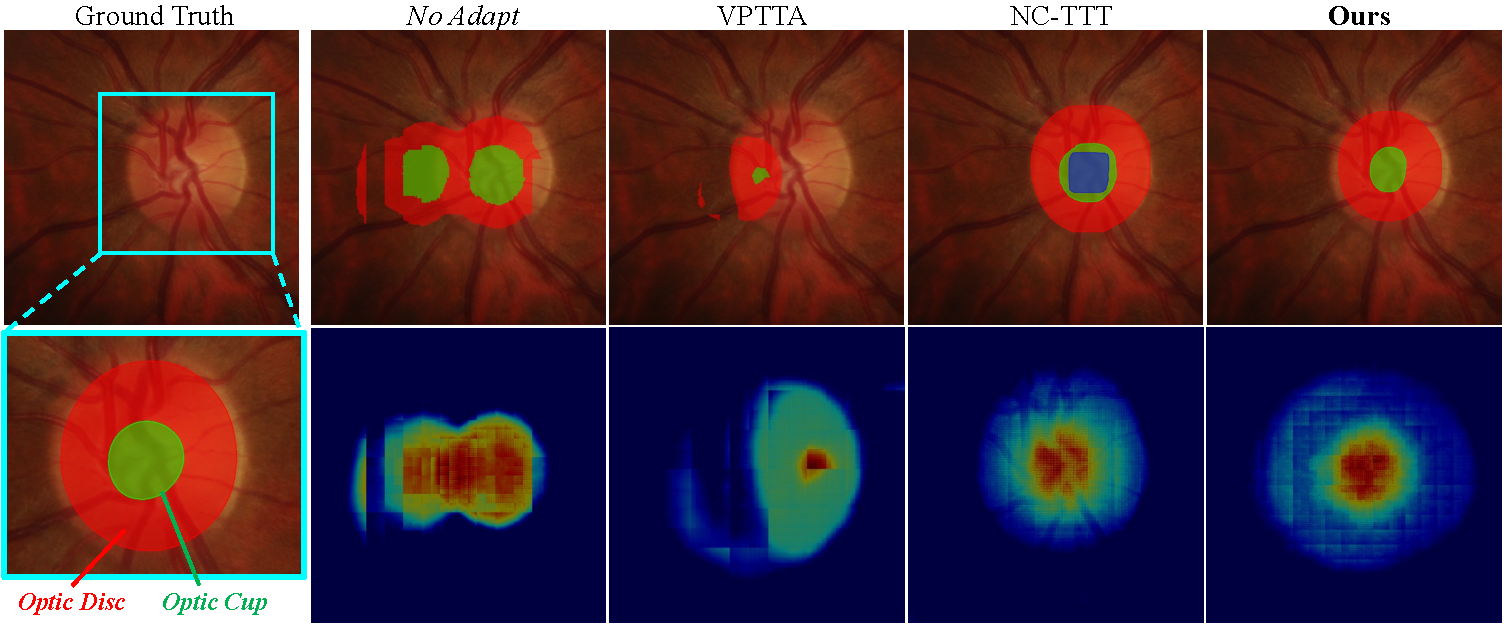
\includegraphics[width=0.999\linewidth]{Figures/visual_compare.pdf}
    % \vspace{-10pt}
    \caption{Visualization comparison of segmentation results and Grad-CAM outputs from the final layer of the backbone network for the \textit{No Adapt} baseline, VPTTA~\cite{chen2024each}, NC-TTT~\cite{osowiechi2024nc}, and our proposed method on retinal fundus images. Additional visual comparisons are provided in the supplementary material.}
     \vspace{-0.5cm}
    \label{fig:visual}
\end{figure}